\documentclass[11pt,a4paper]{article}
\usepackage[T1]{fontenc}
\usepackage[utf8]{inputenc}
\usepackage{lmodern}
\usepackage{amsmath,amssymb,amsthm,mathtools,mathrsfs}
\usepackage{graphicx,float,xcolor,multicol}
\usepackage[shortlabels]{enumitem}
\usepackage[margin=27mm]{geometry}
\usepackage{microtype,needspace,placeins}
\usepackage{tikz,tikz-cd}
\usetikzlibrary{arrows.meta,calc,positioning,patterns,decorations.pathreplacing}
\usepackage[colorlinks=true,linkcolor=teal,urlcolor=teal,citecolor=teal]{hyperref}
\setlength{\parindent}{0pt}
\setlength{\parskip}{.6em}
\setcounter{secnumdepth}{0}
\allowdisplaybreaks
\raggedbottom
\providecommand{\cross}{\times}
\DeclareUnicodeCharacter{2020}{\ensuremath{\dagger}}
\DeclareMathOperator{\supp}{supp}
\DeclareMathOperator*{\esssup}{ess\,sup}
\providecommand{\chapter}{\section}
\newenvironment{tool}[2]{\subsection*{Tool #1 --- #2}}{}
\newcommand{\ToolRef}[1]{Tool #1}
\newcommand{\FigureTag}[2]{\textit{Figure #1}}
\newcommand{\Result}[1]{\subsection*{#1}}
\newcommand{\Application}[1]{\subsubsection*{Application\if\relax\detokenize{#1}\relax\else\space--- #1\fi}}
\newcommand{\ProofHeading}{\par\textit{Proof.}\space}
\newcommand{\ProofOf}[1]{\par\textit{Proof of #1.}\space}
\newcommand{\RemarkHeading}{\par\textbf{Remark.}\space}
\newcommand{\NoteHeading}{\par\textbf{Note.}\space}
\newcommand{\ExerciseHeading}{\par\textbf{Exercise.}\space}

% Rendering support only; mathematical text is in each independent post.
\usepackage{booktabs,array,longtable}
\definecolor{HandoutBlue}{HTML}{2F6690}
\definecolor{HandoutNavy}{HTML}{17365D}
\newtheorem{theorem}{Theorem}
\newtheorem{lemma}[theorem]{Lemma}
\newtheorem{proposition}[theorem]{Proposition}
\newtheorem{corollary}[theorem]{Corollary}
\newtheorem{conjecture}[theorem]{Conjecture}
\newtheorem{definition}{Definition}
\newtheorem{example}{Example}
\newtheorem{namedtoolcounter}{Tool}
\newenvironment{namedtool}[1]{\begin{namedtoolcounter}[#1]}{\end{namedtoolcounter}}
\newtheorem*{claim}{Claim}
\newtheorem*{remark}{Remark}
\newtheorem*{exercise}{Exercise}
\newtheorem*{question}{Question}
\newtheorem*{observation}{Observation}
\newcommand{\SourceChapter}[2]{\section*{#2}}
\newcommand{\Lecture}[2]{\section*{Lecture #1: #2}}
\newcommand{\unclear}[1]{\textit{[unclear: #1]}}
\newcommand{\sourcegap}{\textit{[unfinished in the source]}}
\DeclareMathOperator{\dist}{dist}
\DeclareMathOperator{\id}{id}
\DeclareMathOperator{\Hol}{Hol}
\DeclareMathOperator{\Per}{Per}
\DeclareMathOperator{\Fix}{Fix}
\DeclareMathOperator{\diam}{diam}
\DeclareMathOperator{\Var}{Var}
\DeclareMathOperator{\Leb}{Leb}
\DeclareMathOperator{\Hom}{Hom}
\DeclareMathOperator{\End}{End}
\DeclareMathOperator{\Ann}{Ann}
\DeclareMathOperator{\Spec}{Spec}
\DeclareMathOperator{\Max}{Max}
\DeclareMathOperator{\Ob}{Ob}
\DeclareMathOperator{\Tor}{Tor}
\DeclareMathOperator{\Ass}{Ass}
\DeclareMathOperator{\Mor}{Mor}
\DeclareMathOperator{\Fun}{Fun}
\DeclareMathOperator{\Nat}{Nat}
\DeclareMathOperator{\Cone}{Cone}
\DeclareMathOperator{\MCG}{MCG}
\DeclareMathOperator{\Aut}{Aut}
\DeclareMathOperator{\Deck}{Deck}
\DeclareMathOperator{\SL}{SL}
\DeclareMathOperator{\PSL}{PSL}
\DeclareMathOperator{\Area}{Area}
\DeclareMathOperator{\im}{im}
\DeclareMathOperator{\PSh}{PSh}
\newcommand{\CRing}{\mathsf{CRings}}
\newcommand{\AMod}{A\text{-}\mathsf{Mod}}
\newcommand{\Ab}{\mathsf{Ab}}
\newcommand{\Z}{\mathbb Z}
\newcommand{\Q}{\mathbb Q}
\newcommand{\R}{\mathbb R}
\newcommand{\C}{\mathbb C}
\newcommand{\N}{\mathbb N}
\newcommand{\kk}{\mathbb k}
\renewcommand{\aa}{\mathfrak a}
\newcommand{\bb}{\mathfrak b}
\newcommand{\pp}{\mathfrak p}
\newcommand{\qq}{\mathfrak q}
\newcommand{\mm}{\mathfrak m}
\newcommand{\nn}{\mathfrak n}
\newcommand{\rad}{\mathrm r}
\newcommand{\cat}[1]{\mathsf{#1}}
\setcounter{secnumdepth}{0}
\allowdisplaybreaks

\graphicspath{{figures/ergodic-theory/}}
\begin{document}
\section*{Invariant Measures and the Geometry of Ergodicity}
% BLOG-CONTENT-BEGIN
Let's put both a topological structure and a measure on our state space $X$.

Let $(X,d)$ be a compact metric space and $T\colon X\to X$ be a continuous map. This is the setup of a \emph{topological dynamical system}. It turns out that, the moment you have this, there are some measures you can impose on $X$ naturally, which is precisely why we studied measure-preserving systems first. We want our measures to capture the ``size'' of sets, so we require our measures to be positive. Riesz's representation theorem tells you that all positive linear functionals in $C(X)^*$ are in one-to-one correspondence with bounded Borel measures on $X$:
\[
 \boxed{\Lambda\in C(X)^*\ \sim\ \int_X d\mu,
 \qquad \mu\text{ a bounded Borel measure}.}
\]
Thus, the set of all possible Borel probability measures that one can impose on $X$ can be naturally obtained from the structure imposed on $X$, i.e. the structure of a compact metric space.

Denote by $\mathcal M(X)$ the space of Borel probability measures on $X$. Our
% Source page 2
attempts at building a geometric perspective on ergodicity begin by endowing $\mathcal M(X)$, again, with a natural metric-space structure.

Give $C(X)^*$ the weak-$*$ topology. Notice first that the set
\[
 \mathcal M(X):=\left\{\mu\in C(X)^*\ \middle|\
 \int_X1\,d\mu=1,\quad
 \int_Xf\,d\mu\geq0\text{ for every }f\in C(X),\ f\geq0\right\}
\]
is closed in $C(X)^*$, under the natural identification, because we have:
\begin{itemize}
 \item If $\mu_n\to\mu$, then $\int_X f\,d\mu_n\to\int_X f\,d\mu$ for every $f\in C(X)$. Set $f=1$ to get $\int_X1\,d\mu=1$.
 \item Since $\int_Xf\,d\mu_n\geq0$ and $\int_Xf\,d\mu_n\to\int_Xf\,d\mu$, we get $\int_Xf\,d\mu\geq0$ for every $f\in C(X)$ with $f\geq0$.
\end{itemize}
Clearly, the norm of the operator $\mu$ is $\mu(X)$, for
\[
 \left|\int_Xf\,d\mu\right|\leq\|f\|_\infty\int_X1\,d\mu
\]
(now set $f=1$). Thus $\mathcal M(X)$ is compact in the weak-$*$ topology: by the Banach--Alaoglu theorem, the unit ball in $C(X)^*$, under the usual operator norm, is weak-$*$ compact, and $\mathcal M(X)$ is closed in the unit ball. Further, if $\mu_1,\mu_2\in\mathcal M(X)$, then $s\mu_1+(1-s)\mu_2\in\mathcal M(X)$, so $\mathcal M(X)$ is a convex compact subspace of $C(X)^*$.
% Source omits the range of s in the convex-combination assertion; retained.

\begin{remark}
$\mathcal M(X)$ can also be metrizable, but that aspect of it is not relevant
% Source page 3
to us as of now.
\end{remark}

Given a topological dynamical system $(X,d,T)$, we have a way to associate probability measures on $X$ using the topological structure imposed on $X$. Of these, let us now look at those measures $\mu\in\mathcal M(X)$ such that $\mu$ is $T$-invariant. Then we shall have a measure-preserving system to which we can export our knowledge developed so far.

The map $T$ induces a continuous map $T_*\colon\mathcal M(X)\to\mathcal M(X)$, defined by
\[
 T_*(\mu)(A):=\mu(T^{-1}(A)).
\]
It is continuous because $\int_Xf\,d(T_*\mu)=\int_Xf\circ T\,d\mu$. If $\mu_n\xrightarrow{*}\mu$, then $\int_Xf\circ T\,d\mu_n\to\int_Xf\circ T\,d\mu$, so
\[
 \int_Xf\,d(T_*\mu_n)\longrightarrow\int_Xf\circ T\,d\mu
 =\int_Xf\,d(T_*\mu)
 \qquad\text{for every }f\in C(X).
\]
Hence $T_*\mu_n\to T_*\mu$.

If $\mathcal M^T(X):=\{\mu\in\mathcal M(X)\mid\mu\text{ is $T$-invariant}\}$, the continuity of $T_*$ implies that $\mathcal M^T(X)$ is closed, hence compact, in $\mathcal M(X)$. Also, $\mathcal M^T(X)$ is convex. Therefore $\mathcal M^T(X)$ is also a convex compact subspace of $C(X)^*$.

% Source page 4
\setcounter{theorem}{18}\begin{theorem}[Krylov--Bogolyubov]\label{thm:l6-kb}
We can do ergodic theory on $(X,d,T)$: given a topological dynamical system $(X,d,T)$, we have $\mathcal M^T(X)\neq\varnothing$.
\end{theorem}
\begin{proof}
We have $\mathcal M(X)\neq\varnothing$ because $\delta_x\in\mathcal M(X)$, where, for every Borel set $A\subseteq X$,
\[
 \delta_x(A):=\begin{cases}1,&x\in A,\\0,&\text{otherwise}.\end{cases}
\]
The measures $\delta_x$ can be identified with points in $X$. As $\mathcal M(X)$ is convex, if $X$ has at least two points then $\mathcal M(X)$ will be uncountable.

Now let $\nu_n\in\mathcal M(X)$ and set $\mu_n:=\frac1n\sum_{j=0}^{n-1}T_*^j(\nu_n)$. Since $\mathcal M(X)$ is compact, there exists $\mu_{n(j)}\to\mu$. Let $f\in C(X)$. Then
\[
\begin{aligned}
 \left|\int f\circ T\,d\mu_{n(j)}-\int f\,d\mu_{n(j)}\right|
 &=\frac1{n(j)}\left|\int\sum_{i=0}^{n(j)-1}
    (f\circ T^{i+1}-f\circ T^i)\,d\nu_{n(j)}\right|\\
 &=\frac1{n(j)}\left|\int(f\circ T^{n(j)+1}-f)\,d\nu_{n(j)}\right|\\
 &\leq\frac2{n(j)}\|f\|_\infty\longrightarrow0
 \qquad(j\to\infty).
\end{aligned}
\]
% Author check: source telescopes to T^{n(j)+1}, although the sum ends at n(j)-1; retained.
Thus $\int f\circ T\,d\mu=\int f\,d\mu$ for every $f\in C(X)$, implying that $\mu\in\mathcal M^T(X)$. Hence $\mathcal M^T(X)\neq\varnothing$.
\end{proof}

\begin{remark}
Replace $(X,d,T)$ with $(\mathcal M(X),\widetilde d,T_*)$, where $\widetilde d$ is the metric that generates its weak-$*$ topology. By the
% Source page 5
previous theorem, $\mathcal M^{T_*}(\mathcal M(X))\neq\varnothing$, so there exists a $T_*$-invariant measure on $\mathcal M(X)$. Birkhoff's theorem tells us that, given almost every $\nu\in\mathcal M(X)$,
\[
 \widetilde\mu_n=A_n^\nu:=\frac1n\sum_{i=0}^{n-1}U_{T_*}^i f(\nu)
 \longrightarrow f'(\nu),
\]
where $f'$ is $T_*$-invariant. Since $\{\nu\}$ is a Borel set in the metric space $\mathcal M(X)$, set $f=\chi_{\{\nu\}}$. Now
\[
 \int_{\mathcal M(X)}f'\,d\widetilde\nu
 =\int_{\mathcal M(X)}f\,d\widetilde\nu
 =\widetilde\nu(\{\nu\}),
\]
where $\widetilde\nu$ is the $T_*$-invariant measure. Hence $f'=\chi_{\{\nu\}}$ almost everywhere (only if $f'\geq0$).
% Author check: the source uses A_n^nu for an average of f and asserts f'=chi_{nu}; retained.
\end{remark}

Therefore, we have this dual notion in play here: consider the fact that $\mathcal M(X)$ in some sense also contains $X$.
\[
 \boxed{\begin{gathered}\text{Equidistribution theorems}\\\text{in }\mathcal M(X)\end{gathered}
 \quad\approx\quad
 \begin{gathered}\text{Invariant measures}\\\text{on }X\end{gathered}}
\]

Now recall that $\mathcal M^T(X)$ is convex, so one can talk about its extreme points: points in $\mathcal M^T(X)$ which cannot be further broken down into linear, convex combinations of other elements in $\mathcal M^T(X)$. Denote the set of extreme points by $\mathcal E^T(X)$. For measures in $\mathcal E^T(X)$, we have the following lemma.

\setcounter{theorem}{19}\begin{lemma}
If $\mu_1,\mu_2\in\mathcal E^T(X)$ with $\mu_1\neq\mu_2$, then $\mu_1$ and $\mu_2$ are mutually singular, if $\mu_1$ and $\mu_2$ are ergodic. That is, there exist measurable sets $A,B$ such that $A\cap B=\varnothing$, $A\cup B=X$, and $\mu_1(B)=\mu_2(A)=0$.
\end{lemma}
\begin{proof}
This is a very simple consequence of the ergodic theorem.
% Source page 6
For every $f\in C(X)$, by the pointwise ergodic theorem,
\[
 A_n^f(x)\longrightarrow\int f\,d\mu_1\quad(*)
 \qquad\text{and}\qquad
 A_n^f(x)\longrightarrow\int f\,d\mu_2\quad(\star).
\]
Now choose $f\in C(X)$ such that $\int f\,d\mu_1\neq\int f\,d\mu_2$. If $A=\{x\mid(*)\text{ holds}\}$ and $B=\{x\mid(\star)\text{ holds}\}$, then $\mu_1(A)=\mu_2(B)=1$.
\end{proof}

\begin{remark}
One can generalize this to $n$ ergodic measures by induction. All you need is a function $f\in C(X)$ such that $\{\int f\,d\mu_i\}_{i=1}^n$ is a sequence of distinct elements. Since linear functionals on a topological vector space are open maps, if $\Lambda_i$ represents $\int d\mu_i$, then
\[
 E_{ij}:=\{f\mid\Lambda_i f\neq\Lambda_j f\}
\]
is open and dense in $C(X)$. Thus $\bigcap_{i,j}E_{ij}$ is nonempty, as $C(X)$ is a Baire space. Therefore, if $\mathcal M^T(X)$ were pictorially a convex hull of finitely many ergodic extreme points, then the state space $X$ would have a finite decomposition into ergodic components.
% Author check: the source writes intersection over i,j without excluding i=j; retained.
\end{remark}
\begin{figure}[htbp]
 \centering
 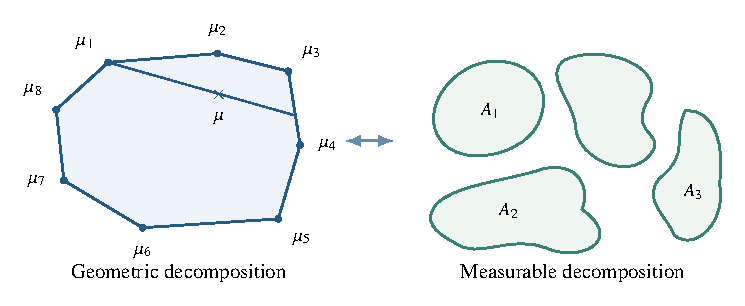
\includegraphics[width=.94\textwidth]{lecture6-fig-01.pdf}
 \FigureTag{L6.1}{fig:lecture6-fig-01}
\end{figure}

% Source page 7
The following theorem ensures that such a geometric decomposition of the space can always be done.
\setcounter{theorem}{20}\begin{theorem}[Extremal Ergodicity]
The ergodic elements of $\mathcal M^T(X)$ are precisely $\mathcal E^T(X)$.
\end{theorem}
\begin{proof}
If $\mu\in\mathcal M^T(X)$ is not ergodic, then there exists $B$ such that $0<\mu(B)<1$ and $T^{-1}B=B$. Thus $\mu(B)^{-1}\mu|_B$ and $\mu(X\setminus B)^{-1}\mu|_{X\setminus B}$ are $T$-invariant, and
\[
 \mu=\mu(B)\bigl(\mu(B)^{-1}\mu|_B\bigr)
 +\mu(X\setminus B)\bigl(\mu(X\setminus B)^{-1}\mu|_{X\setminus B}\bigr),
\]
a convex linear combination.

If $\mu\in\mathcal M^T(X)$ is ergodic and $\mu=s\nu_1+(1-s)\nu_2$, then, since $s,1-s>0$, clearly $\nu_1\ll\mu$ and $\nu_2\ll\mu$. One of these would suffice. The Radon--Nikodym theorem tells you that there exists $f\in L_\mu^1$ such that $f=d\nu_1/d\mu$, implying $\nu_1(A)=\int_Af\,d\mu$.

Here is the cheeky part of the proof. Set $B:=\{x\mid f(x)<1\}$. Then
\[
\begin{aligned}
 \int_{B\cap T^{-1}B}f\,d\mu+\int_{B\setminus T^{-1}B}f\,d\mu
 &=\nu_1(B)=\nu_1(T^{-1}B)\\
 &=\int_{B\cap T^{-1}B}f\,d\mu+\int_{T^{-1}B\setminus B}f\,d\mu,
\end{aligned}
\]
so $\int_{B\setminus T^{-1}B}f\,d\mu=\int_{T^{-1}B\setminus B}f\,d\mu$.

% Source page 8
Also,
\[
\begin{aligned}
 \mu(T^{-1}B\setminus B)
 &=\mu(T^{-1}B)-\mu(T^{-1}B\cap B)\\
 &=\mu(B)-\mu(T^{-1}B\cap B)=\mu(B\setminus T^{-1}B).
\end{aligned}
\]
Now we further have
\[
 \mu(B\setminus T^{-1}B)
 >\int_{B\setminus T^{-1}B}f\,d\mu
 =\int_{T^{-1}B\setminus B}f\,d\mu
 \geq\mu(T^{-1}B\setminus B).
\]
This implies $\mu(B\mathbin\triangle T^{-1}B)=0$, so $\mu(B)\in\{0,1\}$. If $\mu(B)=1$, then
\[
 1=\nu_1(X)=\int_Xf\,d\mu<\mu(B)=1,
\]
a contradiction. Hence $\mu(B)=0$. Similarly, $\mu(\{x\mid f(x)>1\})=0$, so $f(x)=1$ almost everywhere. Thus $\nu_1=\mu$, implying $\mu\in\mathcal E^T(X)$: it is an extreme point.
\end{proof}

The argument made in the remark above can be extended to a countable collection of elements in $\mathcal E^T(X)$. In such cases, using the ergodic theorem, one can get an explicit decomposition of the state space. But a more interesting question is: what about the case when $\mathcal E^T(X)$ is a continuum? How is one supposed to get down to the minimal dynamical nuts and bolts of a given measure-preserving topological dynamical system? In that case, Choquet's representation theorem
% Source page 9
comes in handy to yield ergodic components of the state space as infinitesimal components of an integral representation!

\setcounter{theorem}{21}\begin{theorem}[Ergodic Decomposition]
Given a topological dynamical system $(X,T)$ and any $\mu\in\mathcal M^T(X)$, there exists a unique probability measure $\lambda$ on the Borel sets of $\mathcal M^T(X)$ such that
\[
 \lambda(\mathcal E^T(X))=1,
 \qquad
 \int_Xf\,d\mu=\int_{\mathcal E^T(X)}\left(\int_Xf\,d\nu\right)d\lambda(\nu)
 \quad\text{for all }f\in C(X).
\]
These correspond, respectively, to the finite expressions $\sum_{i=1}^n c_i=1$ and $\mu=\sum_{i=1}^n c_i\nu_i$.
\end{theorem}

\begin{remark}
Notice also that the uniqueness of $\lambda$ tells you that the decomposition is unique!
\end{remark}
% BLOG-CONTENT-END
\end{document}
